%======================================================================
\chapter{Evaluation}
\label{chap:e}
%======================================================================

To evaluate the developed framework, a skill transfer study will be conducted with the following objectives:

\begin{itemize}
	\item
	to analyze the efficiency of the framework as a training tool for skill transfer, and
	\item
	to compare the performance of trainees with those trained using traditional training methods.
\end{itemize}

The evaluation involves two experimental groups:

\begin{itemize}
	\item
	Two-way AR group: participants are trained using the proposed two-way AR training platform.
	\item
	One-way AR group: participants are trained using the one-way AR training platform.
	\item
	Control group: participants are trained using an instructional video.
\end{itemize}

The experimental task is a mortise-and-tenon assembly task. It requires the participants to assemble the mortise-and-tenon parts together in a proper way. We will recruit 45 participants that are assigned into three groups: participants in the AR group will be trained using the proposed two-way AR training platform, participants in the One-way AR group will be trained using the one-way AR training platform, while those in the control group will be trained using an instructional video.

\section{Procedure}

\subsection{Introduction to the task and procedure}

The experimenter will first explain to the participants the purpose of the experiment - namely to evaluate the different training methods for assembly skills transfer.
The general information about the task will be also given to the participants.
Then they will be told that, after the training, they will be asked to accomplish the task on their own as fast as possible and without errors.

\subsection{Introduction to the training method}

Participants in different groups will be given different introduction to the platform they will use.
Participants in the two-way AR training platform and one-way AR training platform will be given instructions on the tablet PC with a touch screen that would serve as the AR platform. They will also be introduced to the program we will develop to use in the training platform.
Participants in the control group will be told that they would perform the training using an instruction video describing the task.

\subsection{Familiarization with the training platform}

For all the three groups, participants will be asked to familiarize the training platform with a pre-task. The pre-task is a burr puzzle that can be treated as a simplified version of the main task, see Figure~\ref{fig:burr-puzzle}.
The left figure of Figure~\ref{fig:burr-puzzle} shows the components of the burr puzzle, and the right figure shows the assembled status of the burr puzzle.

\begin{figure}
	\centering
	\subfigure[Before assembly]{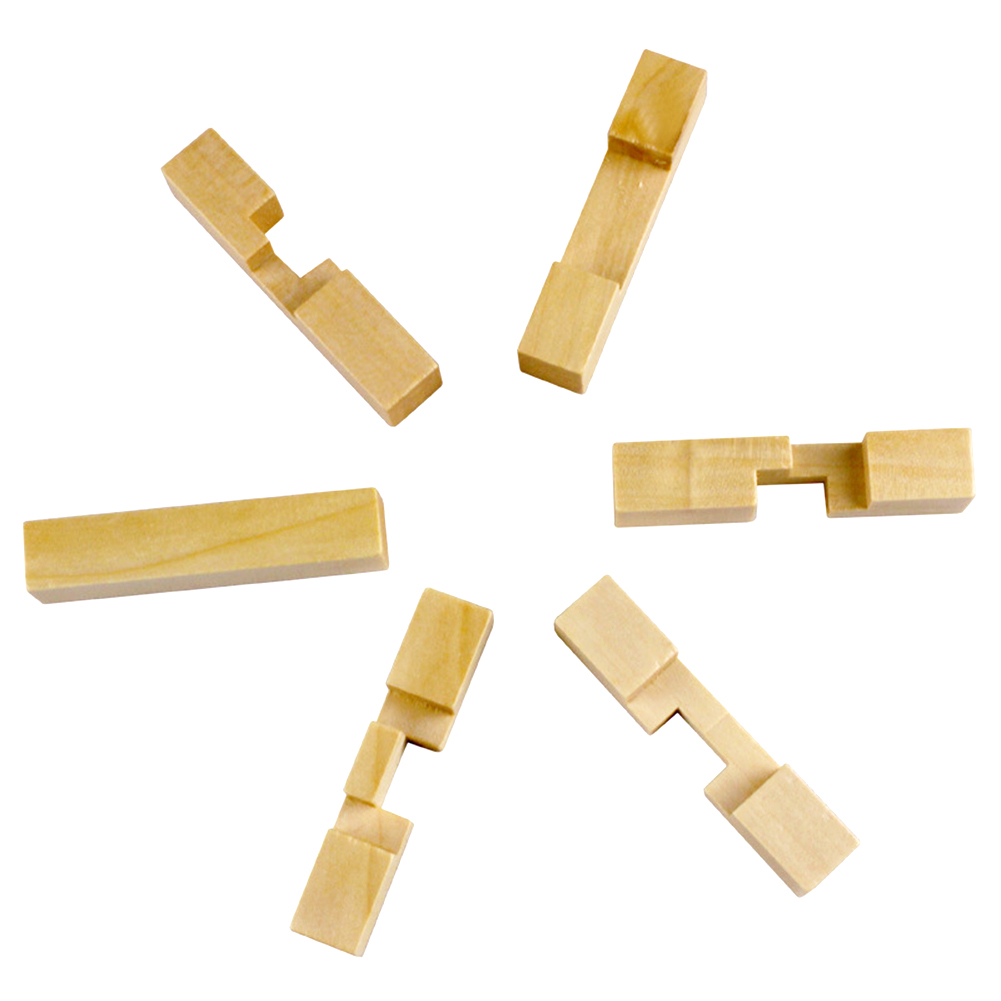
\includegraphics[width=0.35\columnwidth]{figures/burr-puzzle-parts.jpg}}
	\subfigure[After assembly]{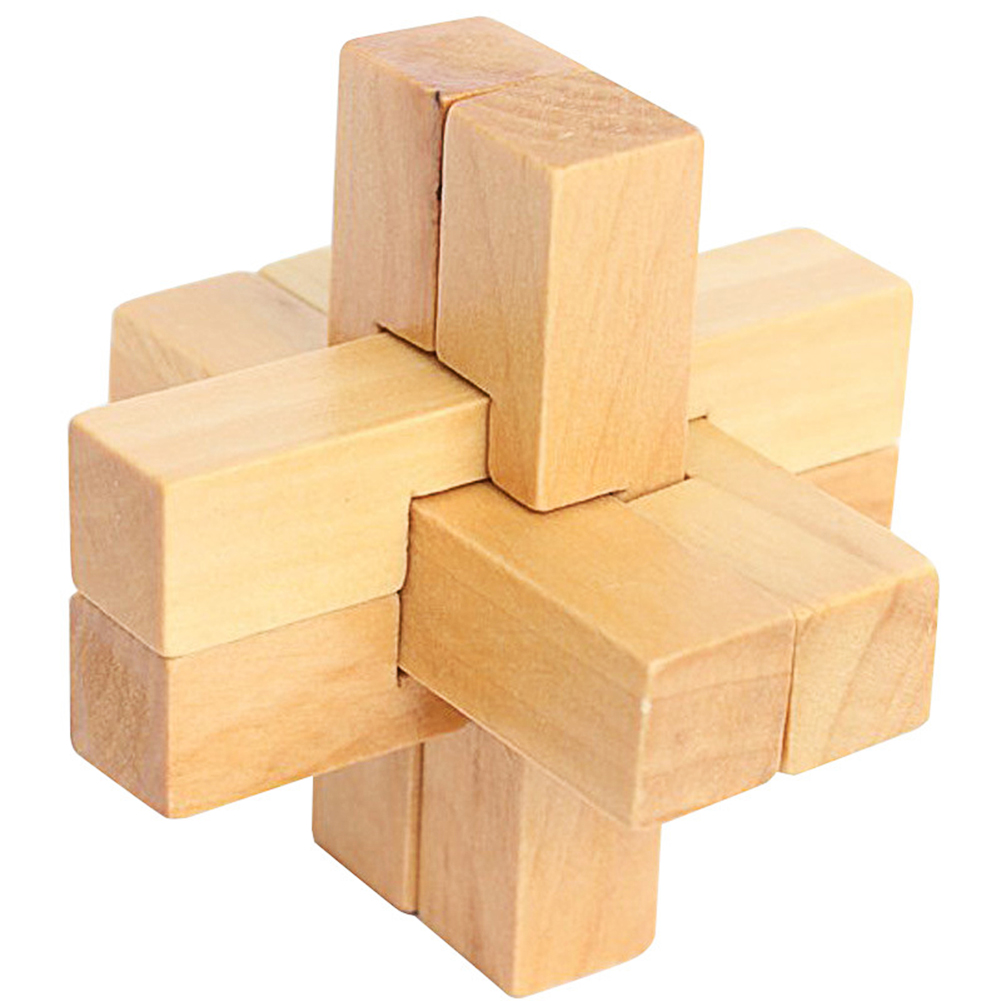
\includegraphics[width=0.35\columnwidth]{figures/burr-puzzle.jpg}}
	\captionsource{Pre-task}{\cite{burr-puzzle}}
	\label{fig:burr-puzzle}
\end{figure}

The participants in all the three groups will be asked to solve the puzzle with the help of the corresponding training method. They will be told that this pre-task is only for them to familiarize the training platform and it is not necessary to solve it if it is too difficult.

\subsection{Training}

After familiarization of the training platform, the training will open with a general explanation of the task, and a reminder to the participants that they will be asked to accomplish the task on their own later.

We choose multi-layer bracket assembly as the mortise-and-tenon task.
The multi-layer bracket is a bracket system used in ancient Chinese architectures.
Figure~\ref{fig:mat-task} demonstrate the multi-layer bracket and its parts. A multi-layer bracket is composed of tens of parts, the parts are connected with each other using mortise-and-tenon joints.

At the beginning of the training, all the parts are detached from each other. The participants will be asked to assemble them with the help of different training platforms.

The participants in the two-way AR group will use the proposed AR training platform, during which the experimenter will act as the remote trainer. The experimenter will perform the task in another room, so that the participants would not to see the experimenter. The participants will follow the live instructions and get the feedback from the experimenter.

The participants in the one-way AR group will use a one-way AR training platform that has pre-defined materials, while the participants in the control group will use an instruction video to learn how to perform the task.

The training time of each participant will be recorded.

\begin{figure}
	\centering
	\subfigure[Multi-layer bracket]{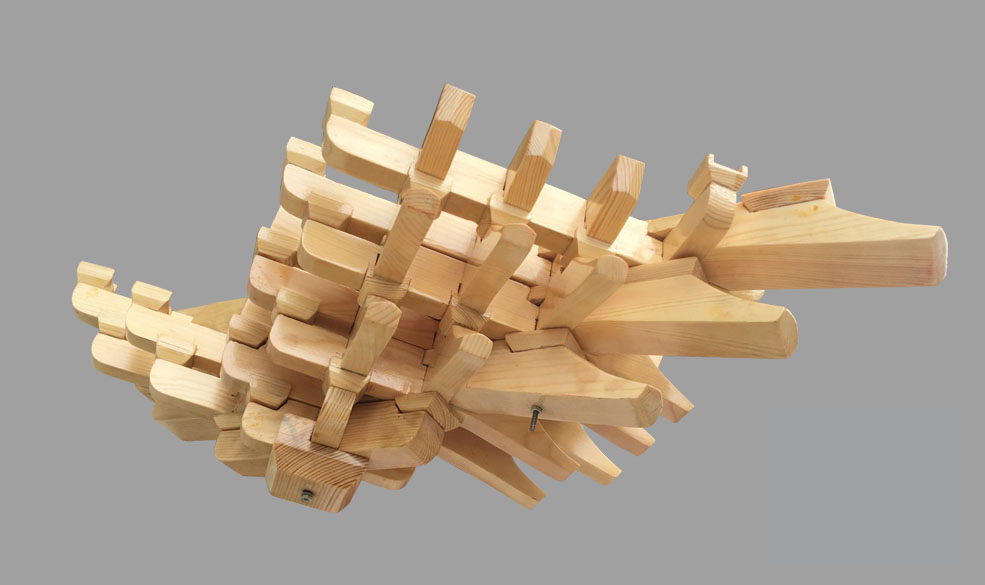
\includegraphics[width=0.35\columnwidth]{figures/bracket.jpg}}
	\subfigure[Parts of the multi-layer bracket]{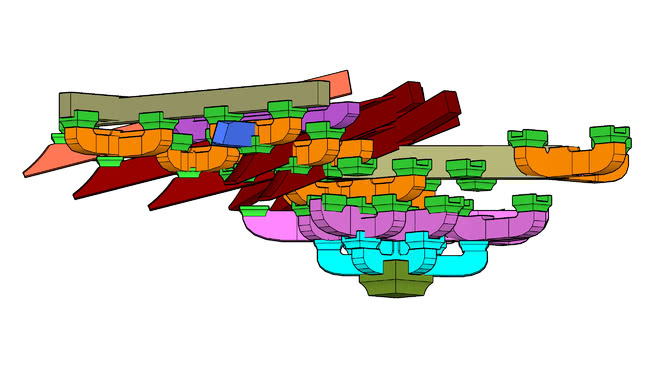
\includegraphics[width=0.35\columnwidth]{figures/bracket-parts.jpg}}
	\centering
	\captionsource{Mortise-and-tenon task}{\cite{ml-bracket-1,ml-bracket-2}}
	\label{fig:mat-task}
\end{figure}

\subsection{Test}

The participants will be asked to perform the task correctly on their own after the training. During the test, if they feel that they could not continue the task, they can ask the experimenter to perform one step for them. However, they will be told that the number of helps from the experimenter indicated the number of solved error, which is one of the measures of their performance.

After the test, we will record the performance time of each participant and inspect the buckets that they assembled to count the number of unsolved errors made by each participant.

\section{Hypothesis}

We devise three null hypothesis to test in the experiment:

\begin{table}[!htbp]
\caption{Hypotheses.}
\label{tab:hypo}
\small{
\begin{tabular}{ll}
\noalign{\smallskip}\hline\noalign{\smallskip}
H\textsubscript{01} & Participants in all the groups have equal performance in performance time \\
H\textsubscript{02} & Participants in all the three groups have equal performance in number of unsolved errors \\
H\textsubscript{03} & Participants in all the three groups have equal performance in number of solved errors \\
\noalign{\smallskip}\hline
\end{tabular}
}
\end{table}

\section{Participants}

45 volunteers will be recruited in the experiment. The number of participants is comparable with similar studies. There are 20 participants in \cite{webel2013}, 24 participants in \cite{wang2010}, 40 participants in \cite{gavish2015}, and 6 participants in \cite{henderson2009}. We will make sure that all the participants do not have experience on the mortise-and-tenon task.

\section{Independent Variables and Dependent Measures}

The experiment will be conducted with three independent variables: training method. It has three levels: two-way AR training platform, one-way AR training platform, and instruction video.

In the experiment, we will collect three types of data: performance time, number of solved errors, and number of unsolved errors.
The performance time indicates the time period during which the participants accomplish the task.
Number of solved errors is the numbers of helps the participant got from the experimenter.
Number of unsolved errors indicates the number of errors on the finished product.

\section{Analysis}

After the experiment, we can calculate the mean values for all the three measures and groups. However, to understand the result statistically, we use analysis of variance (ANOVA) to interpret our experiment results.

Since there is only one independent variable, training method, we use one-way ANOVA test to investigate the effect of the factor. We compare the $p$-value to a significance level to decide whether the null hypothesis should be rejected. We choose a significance level of 0.05.
